\section{Theory}
The restricted Boltzmann machine (RBM) is an energy-based model defined by the energy function~\cite{goodfellow_deep_learning}
\begin{align}
\begin{split}
    \label{eq:rbm_energy}
    E(\vec{v}, \vec{h})
        &= -\sum_{i=1}^{n_v} a_i v_i - \sum_{j=1}^{n_h} b_j h_j - \sum_{i=1}^{n_v} \sum_{j=1}^{n_h} v_i w_{ij} h_j \\
        &= -\vec{a}^\intercal\vec{v} - \vec{b}^\intercal\vec{h} - \vec{v}^\intercal\mat{W}\vec{h},
\end{split}
\end{align}
where
\begin{itemize}
    \item \( \vec{v} \in \binset^{n_v} \) represents the visible units, with associated bias vector \( \vec{a} \in \R^{n_v} \).
    \item \( \vec{h} \in \binset^{n_h} \) represents the hidden units, with associated bias vector \( \vec{b} \in \R^{n_h} \).
    \item \( \mat{W} \in \R^{n_v \times n_h} \) represents the weights corresponding to the interaction strengths between visible and hidden units.
\end{itemize}

\begin{figure}[!htb]
    \begin{center}
        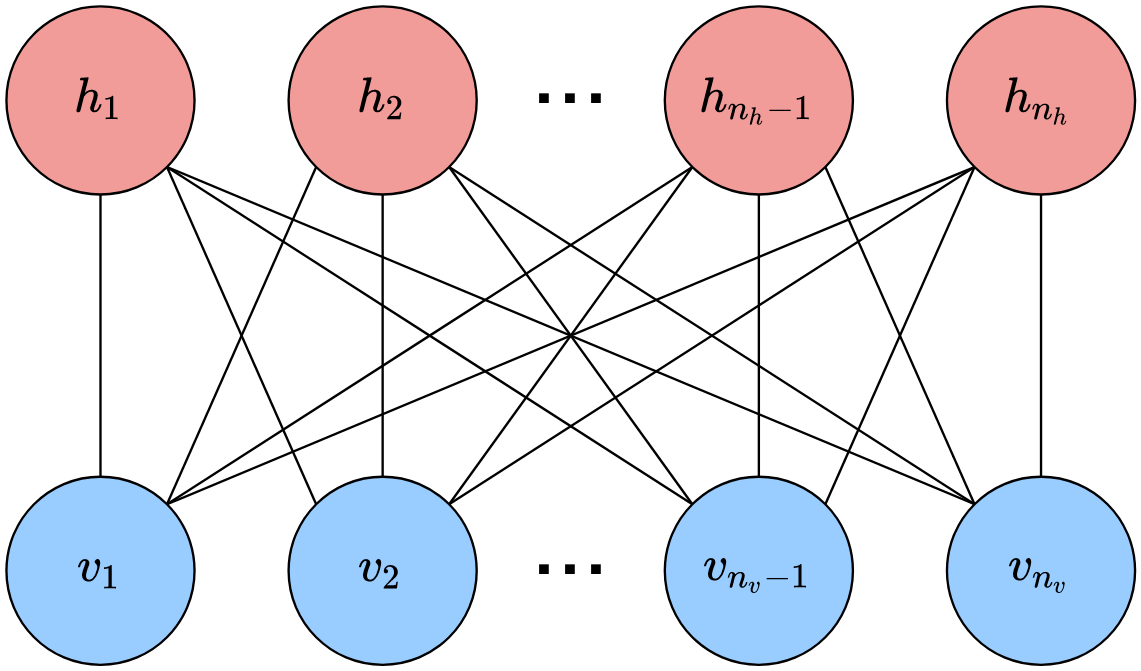
\includegraphics[width=1\linewidth]{rbm_diagram.png}
    \end{center}
    \caption{Diagram of a restricted Boltzmann machine with \( n_v \) visible units and \( n_h \) hidden units.}
    \label{fig:rbm_diagram}
\end{figure}

It is termed \textit{restricted} due to the fact that there are no intra-layer connections, i.e., visible units are only connected to hidden units, and vice versa.
An example diagram is depicted in~\cref{fig:rbm_diagram}.

The probability to find the system in the configuration \( (\vec{v},\vec{h}) \) is given by the Boltzmann distribution (with \( \beta = 1/kT = 1 \))
\begin{align}
    \label{eq:rbm_joint_probability}
    p(\vec{v}, \vec{h}) = \frac{1}{Z} e^{-E(\vec{v},\vec{h})},
\end{align}
with intractable~\cite{long_servedio_2010} partition function
\begin{align}
    \label{eq:rbm_partition_function}
    Z = \sum_{\vec{v},\vec{h}} e^{-E(\vec{v},\vec{h})},
\end{align}
where \( \sum_{\vec{v},\vec{h}} \) denotes the sum over all possible configurations of \( \vec{v} \) and \( \vec{h} \).

The imposed restrictions on intra-layer connections enable us to write the conditional probabilities of the layers as the product of the individual units' probabilities~\footnote{Here \( \sigma(x) \) is the element-wise logistic sigmoid function and \( \odot \) denotes element-wise multiplication.} (see \cref{app:conditional_probabilities_derivation} for derivation)
\begin{align}
\begin{split}
    p(\vec{h} | \vec{v})
        &= \prod_{j=1}^{n_h} \sigma\big( (2\vec{h} - 1) \odot (\vec{b} + \mat{W}^\intercal\vec{v}) \big)_j, \\
    p(\vec{v} | \vec{h})
        &= \prod_{i=1}^{n_v} \sigma\big( (2\vec{v} - 1) \odot (\vec{a} + \mat{W}\vec{h}) \big)_i.
\end{split}
\end{align}

\subsection{Optimizing an RBM}
Due to the intractability of the partition function, the model cannot be solved exactly in general, thus we resort to other methods to optimize it such as likelihood maximization via gradient descent.
For data set distribution \( p_\text{data} \) and parameters \( \theta = (\mat{W}, \vec{a}, \vec{b}) \), the log-likelihood is given by
\begin{align}
\begin{split}
    \ell(\theta)
        &= \sum_{\vec{v}} p_{\text{data}}(\vec{v}) \log p(\vec{v}) \\
        &= \sum_{\vec{v}} p_{\text{data}}(\vec{v}) \log \bigg(\frac{1}{Z} \sum_\vec{h} e^{-E(\vec{v},\vec{h})}\bigg),
\end{split}
\end{align}
with gradients (see \cref{app:rbm_log_likelihood_derivation} for derivation)
\begin{align}
\begin{split}
    \partial_{w_{ij}} \ell(\theta)
        &= \langle v_i h_j \rangle_{\text{data}} - \langle v_i h_j \rangle_{\text{model}}, \\
    \partial_{a_i} \ell(\theta)
        &= \langle v_i \rangle_{\text{data}} - \langle v_i \rangle_{\text{model}}, \\
    \partial_{b_j} \ell(\theta)
        &= \langle h_j \rangle_{\text{data}} - \langle h_j \rangle_{\text{model}}.
\end{split}
\end{align}

The part of the gradient using the data set distribution is referred to as the \textit{positive} phase, and the part using the model distribution is referred to as the \textit{negative} phase.
It is trivial to compute the expectation values in the positive phase, but not so much in the negative phase because \( p(\vec{v}) \) cannot be sampled directly.

In practice the negative phase expectation values are sampled using a Markov chain Monte Carlo (MCMC) method.
This is done via Gibbs sampling~\cite{hinton_rbm_training}, which uses the conditional probabilities \( p(\vec{h}|\vec{v}) \) and \( p(\vec{v}|\vec{h}) \).
One starts with a visible vector and then samples the hidden units conditioned on the visible units, followed by sampling the visible units conditioned on the hidden units, and so forth until the desired thermalization threshold is reached.
The number of steps required to reach thermalization is model dependent and can be estimated by analyzing the autocorrelations of a sample chain generated by the model.
The algorithm for Gibbs sampling is given in \cref{alg:Gibbs} and illustrated in \cref{fig:gibbs_sampling_diagram}.
The algorithm is presented in a vectorized format for brevity.

\begin{algorithm}
\caption{Gibbs Sampling}
\begin{algorithmic}[1]
    \Procedure{Gibbs}{$\vec{v},n,\mat{W},\vec{a},\vec{b}$}
        \State $n_v \gets$ length$(\vec{a})$
        \State $n_h \gets$ length$(\vec{b})$
        \For{$k$ in 1 to $n$}
            \State $\vec{r} \sim$ Uniform$(0, 1, n_h)$
            \State $\vec{h} \gets \vec{r} < \sigma(\vec{b} + \mat{W}^\intercal\vec{v})$
                \Comment $\sigma, <$ applied element-wise
            \State $\vec{r} \sim$ Uniform$(0, 1, n_v)$
            \State $\vec{v} \gets \vec{r} < \sigma(\vec{a} + \mat{W}\vec{h})$
                \Comment $\sigma, <$ applied element-wise
        \EndFor
        \State \Return $\vec{v}$
    \EndProcedure
\end{algorithmic}
\label{alg:Gibbs}
\end{algorithm}
The Uniform$(a, b, n)$ function in \cref{alg:Gibbs} produces a length \( n \) vector of uniform i.i.d. random variables on the interval $[a, b)$, and the \( < \) operator returns a binary output with \( (\text{true}, \text{false}) \mapsto (1, 0) \).

\begin{figure}
    \begin{center}
        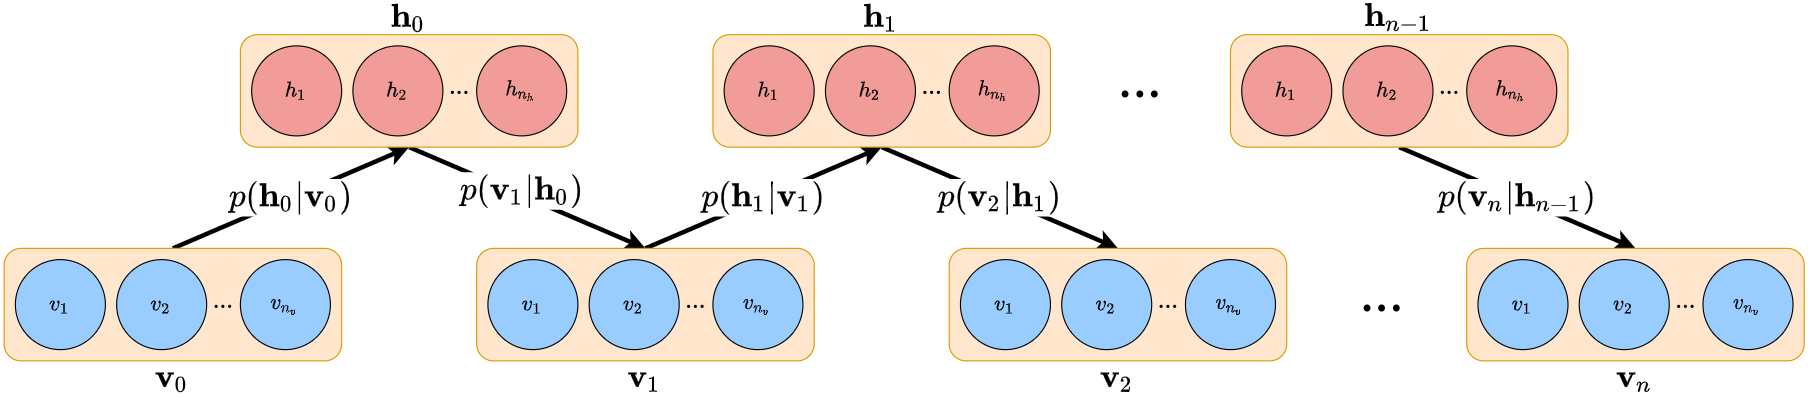
\includegraphics[width=1\linewidth]{gibbs_sampling_diagram.png}
    \end{center}
    \caption{Illustration of the \( n \)-step Gibbs sampling procedure.}
    \label{fig:gibbs_sampling_diagram}
\end{figure}

The standard procedure for training an RBM is called \( n \)-step contrastive divergence (CD-\( n \)), with \( n \) often taken to be one in practice~\cite{hinton_rbm_training}.
The algorithm is detailed in \cref{alg:CDn}, where one can see that \( n \) corresponds to how many Gibbs sampling steps are between the positive and negative phase gradients.
Applying the algorithm to a mini-batch is essentially the same except that one divides the learning rate by the size of the mini-batch to get a mini-batch averaged gradient.

\begin{algorithm}
\caption{$n$-Step Contrastive Divergence (CD-$n$)}
\begin{algorithmic}[1]
    \Procedure{CD}{$\vec{v}_+,n,\mat{W},\vec{a},\vec{b},\eta$}
        \Comment $\vec{v}_+$ is a training sample
        \State $\vec{h}_+ \gets \sigma(\vec{b} + \mat{W}^\intercal\vec{v}_+)$
            \Comment $\sigma$ applied element-wise
        \State $\vec{v}_- \gets$ Gibbs$(\vec{v}_+,n,\mat{W},\vec{a},\vec{b})$
        \State $\vec{h}_- \gets \sigma(\vec{b} + \mat{W}^\intercal\vec{v}_-)$
            \Comment $\sigma$ applied element-wise
        \State $\mat{W} \gets \mat{W} + \eta(\vec{v}_+ \vec{h}_+^\intercal - \vec{v}_- \vec{h}_-^\intercal)$
        \State $\vec{a} \gets \vec{a} + \eta(\vec{v}_+ - \vec{v}_-)$
        \State $\vec{b} \gets \vec{b} + \eta(\vec{h}_+ - \vec{h}_-)$
        \State \Return $\mat{W}, \vec{a}, \vec{b}$
    \EndProcedure
\end{algorithmic}
\label{alg:CDn}
\end{algorithm}


\section{The Classical Market Generator}\label{sec:classical_market_generator}
In \textit{The Market Generator}~\cite{kondratyev_2019} by Kondratyev and Schwarz, they show how an RBM can be used as a generative model to produce synthetic market data.
Specifically, they study how it performs on the log returns of forex data for the same currency pairs we use here for the time period 1999-2019.
In this section we use some of the same metrics, as well as a couple additional ones, so that we can verify our models achieve similar performance to theirs, as well as give us a good reference point to compare our quantum models within~\cref{ch:qbm}.

\subsection{Models}
We train and analyze four RBM models using variations of the filtered data set from~\cref{ch:data_analysis}, each with slightly different preprocessing procedures denoted by:
\begin{itemize}
    \item (B): base data set.
    \item (X): base data set transformed using~\cref{alg:transformation}.
    \item (V): base data set with additional volatility indicators.
    \item (XV): base data set transformed using~\cref{alg:transformation} with additional volatility indicators.
\end{itemize}
The models here have 64 (68 for ones with volatility indicators) visible units and 30 hidden units (the same as in~\cite{kondratyev_2019}) to act as regularized autoencoders.
We use a mini-batch size of 10, and an initial learning rate of \( 10^{-3} \) that decays by a factor of half every 1000 epochs after epoch 5000 as defined in~\cref{app:lr_exp_decay}, for a total of \( 10^4 \) epochs.
We base the models on a modified version of scikit-learn's~\cite{python_sklearn} BernoulliRBM class, which we forked~\footnote{https://github.com/cameronperot/scikit-learn/} to implement the ability to use a learning rate schedule with the BernoulliRBM class.

One of the drawbacks of the RBM is that it is not easy to track the training progress for our use case, as the pseudolikelihood metric implemented by the scikit-learn package is not necessarily a good proxy for our models' performances.
The Kullback-Leibler (KL) divergence of \( \pmodel \) from \( \pdata \), denoted \( \DKL{\pdata}{\pmodel} \), is a suitable quantity to track model performance as it measures the information loss associated with using the model distribution \( \pmodel \) to approximate the data set distribution \( \pdata \) (more information in~\cref{app:kl_divergence}).
However, due to the high number of epochs and the thermalization requirements of samples generated by the RBM, this is not very feasible because generating samples to compute the KL divergence every epoch significantly increases model training times.
Therefore, we only present the final results of the models.

\subsection{Results}
\subsubsection{Autocorrelations}
As mentioned before, the classical RBM sampling method is based on an MCMC algorithm, and thus samples produced via this method are autocorrelated.
Therefore, we first examine the autocorrelations to see how dependent samples are on the previous, so that we can get an idea of how many Gibbs steps are needed between samples to consider them statistically independent.
We use Gibbs sample chains of length \( 10^8 \) for this analysis.
More information about the autocorrelation function and time can be found in~\cref{app:autocorrelation_analysis}.

\cref{fig:rbm_autocorrelation_functions} shows the autocorrelation functions for the various models and currency pairs.
It is immediately clear that the autocorrelations fall off much sooner for the models trained on the transformed data sets for all currency pairs.
This observation is confirmed by examining the integrated autocorrelation times in~\cref{tbl:rbm_ac_times}.

It is not immediately clear why the transformed data sets lead to such shorter integrated autocorrelation times, but this is a welcome trend as it means that less sampling steps are required to reach thermalization.
\begin{figure}[!htb]
    \begin{center}
        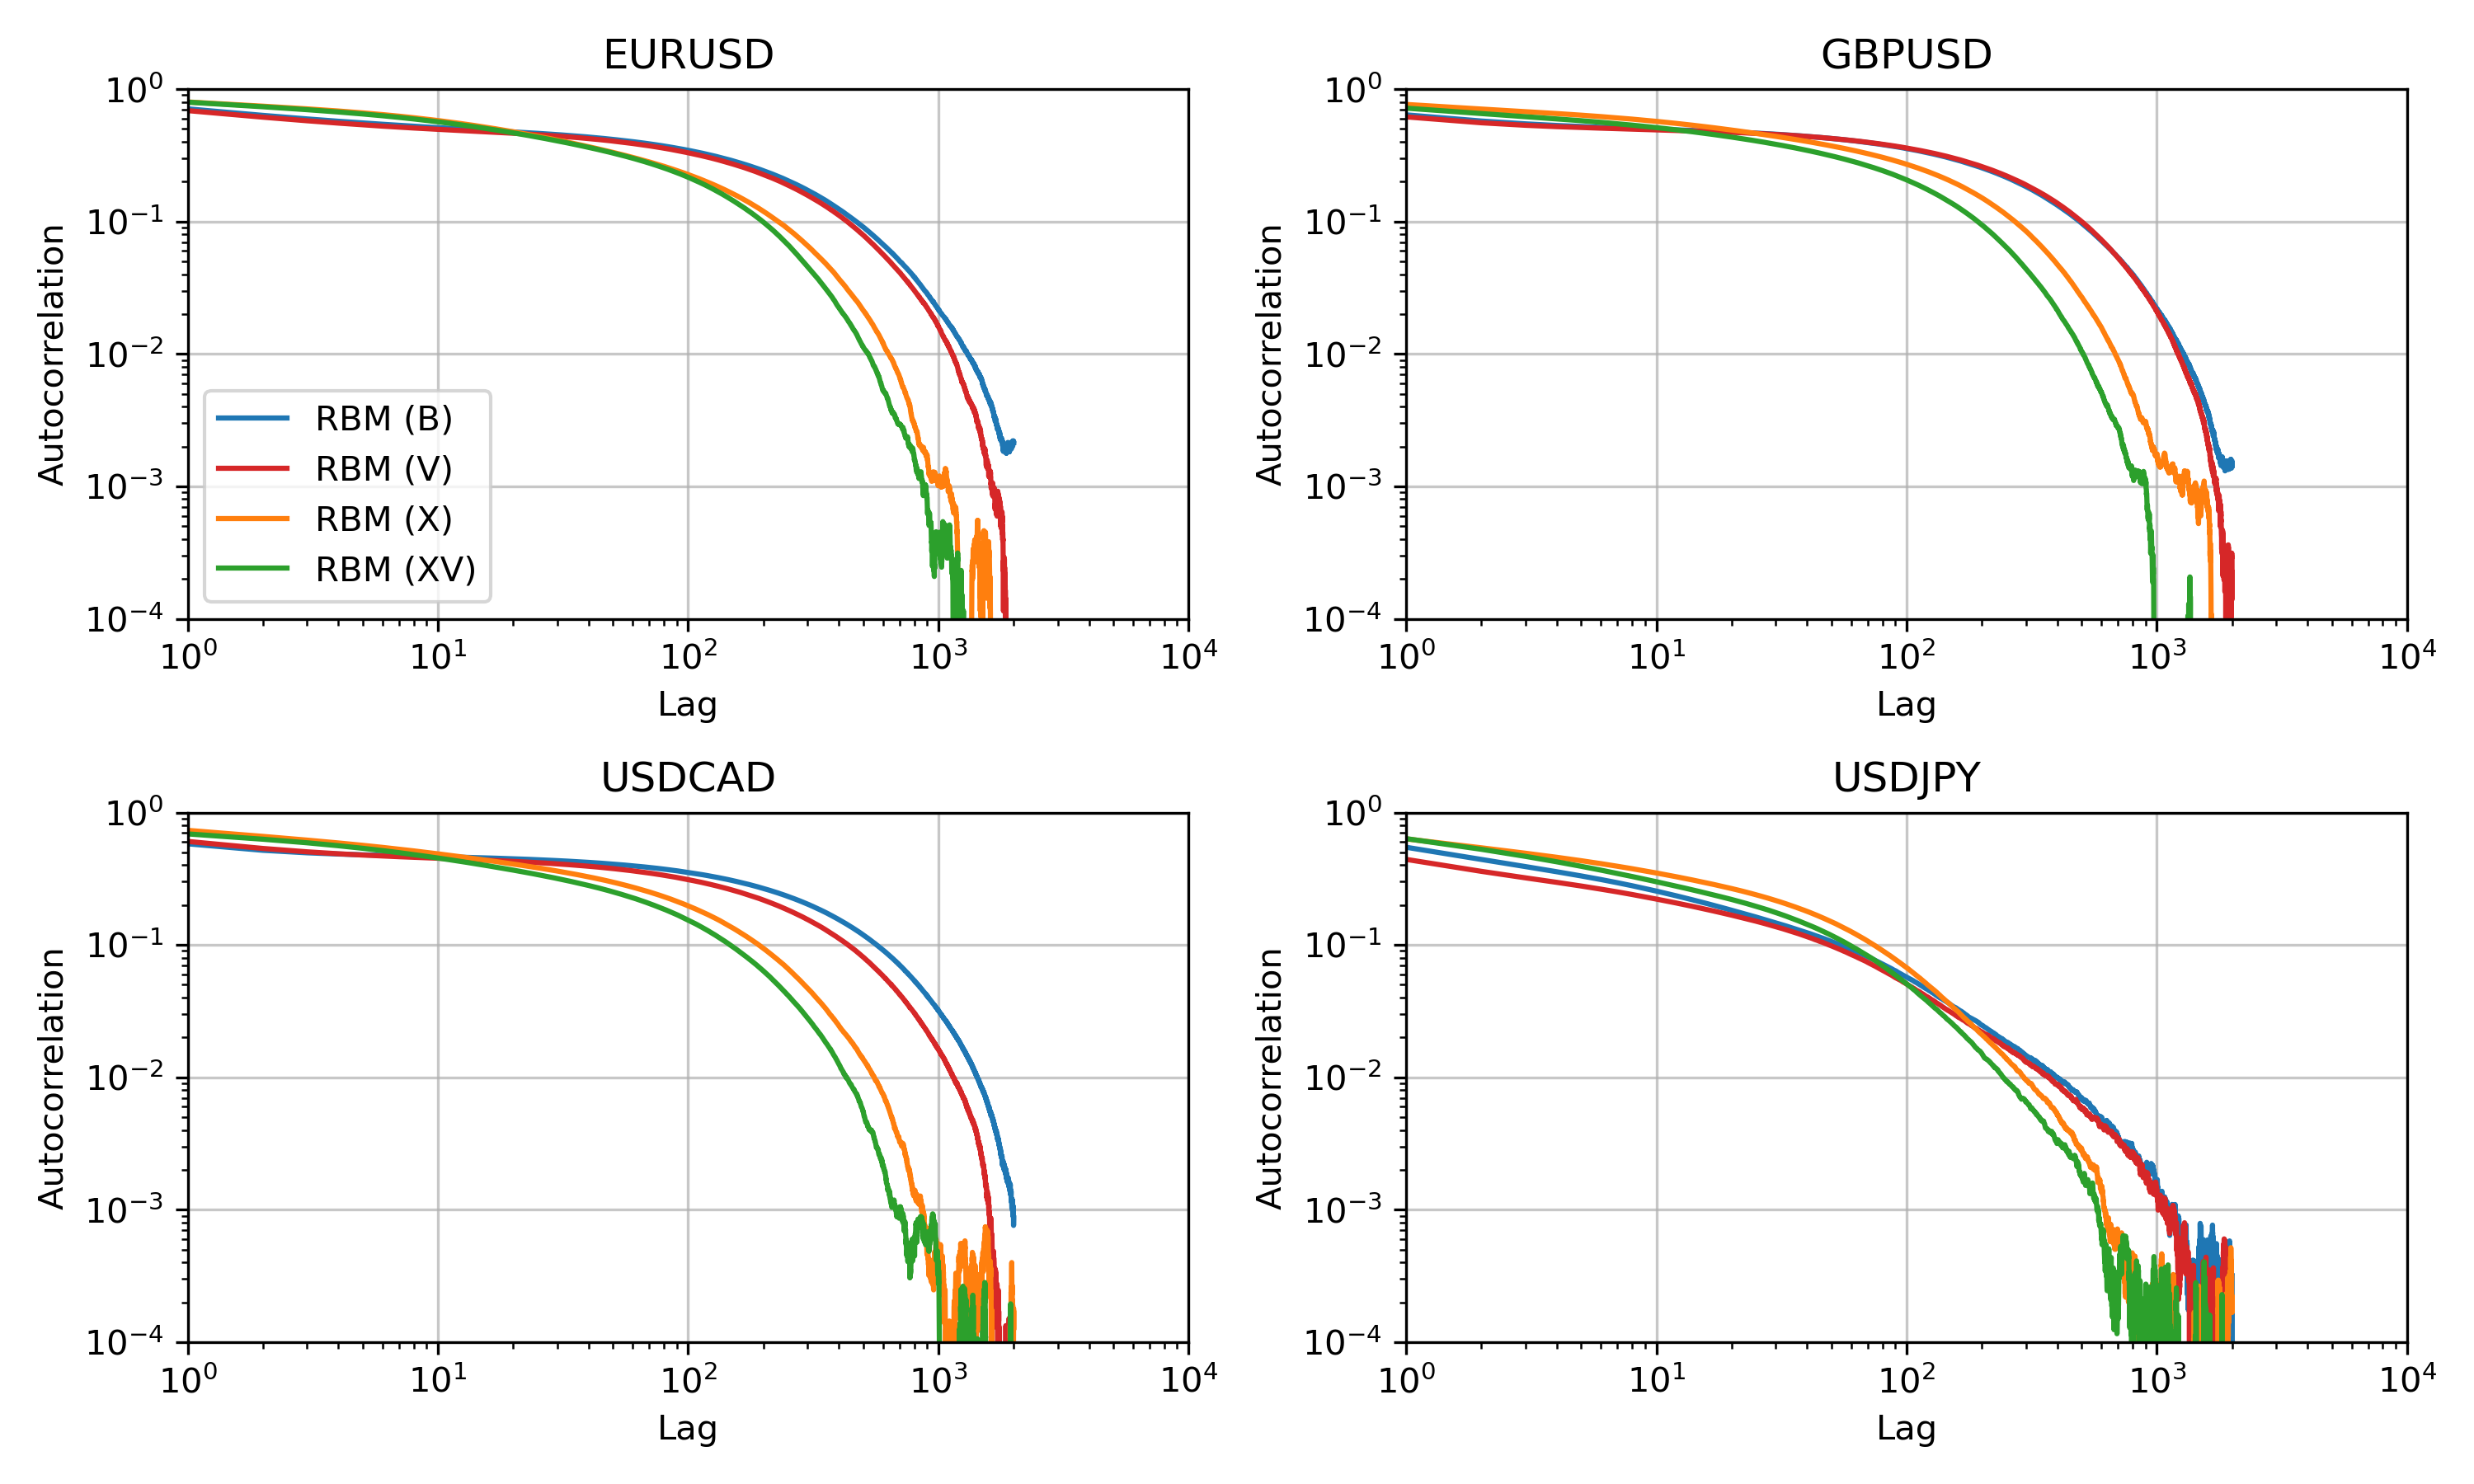
\includegraphics[width=1\linewidth]{rbm/autocorrelation_functions.png}
    \end{center}
    \caption{
        Autocorrelation functions of the RBM models.
    }
    \label{fig:rbm_autocorrelation_functions}
\end{figure}
\begin{table}[!htb]
    \centering
    \begin{adjustbox}{max width=\textwidth}
        \input{../tables/rbm/autocorrelation_times.tbl}
    \end{adjustbox}
    \caption{
        Integrated autocorrelation times of the RBM models.
    }
    \label{tbl:rbm_ac_times}
\end{table}

The results in the rest of this section are derived from an ensemble of 100 sample sets consisting of \( 10^4 \) samples each, and \( 10^4 \) Gibbs sampling steps between samples to ensure thermalization.

\subsubsection{Marginal Distributions}
To get an idea of how well the models perform, we examine the KL divergences of the marginal distributions of each currency pair in~\cref{tbl:rbm_KL_divergences}.
Here we observe that all models reproduce the marginal distributions quite well, but the models trained on the transformed data sets perform slightly better, particularly on the USDCAD marginal.
The performance of the models on the marginal distributions is also visualized with Q-Q plots in~\cref{fig:rbm_qq_plots}.
More information on how the KL divergences are computed can be found in~\cref{app:kl_divergence_in_practice}.
\begin{table}[!htb]
    \centering
    \begin{adjustbox}{max width=\textwidth}
        \input{../tables/rbm/kl_divergences.tbl}
    \end{adjustbox}
    \caption{
        KL divergences of the RBM models.
        The values are shown in the format mean \(\pm\) one standard deviation from an ensemble of 100 sample sets consisting of \( 10^4 \) samples each.
    }
    \label{tbl:rbm_KL_divergences}
\end{table}
\begin{figure}[!htb]
    \begin{center}
        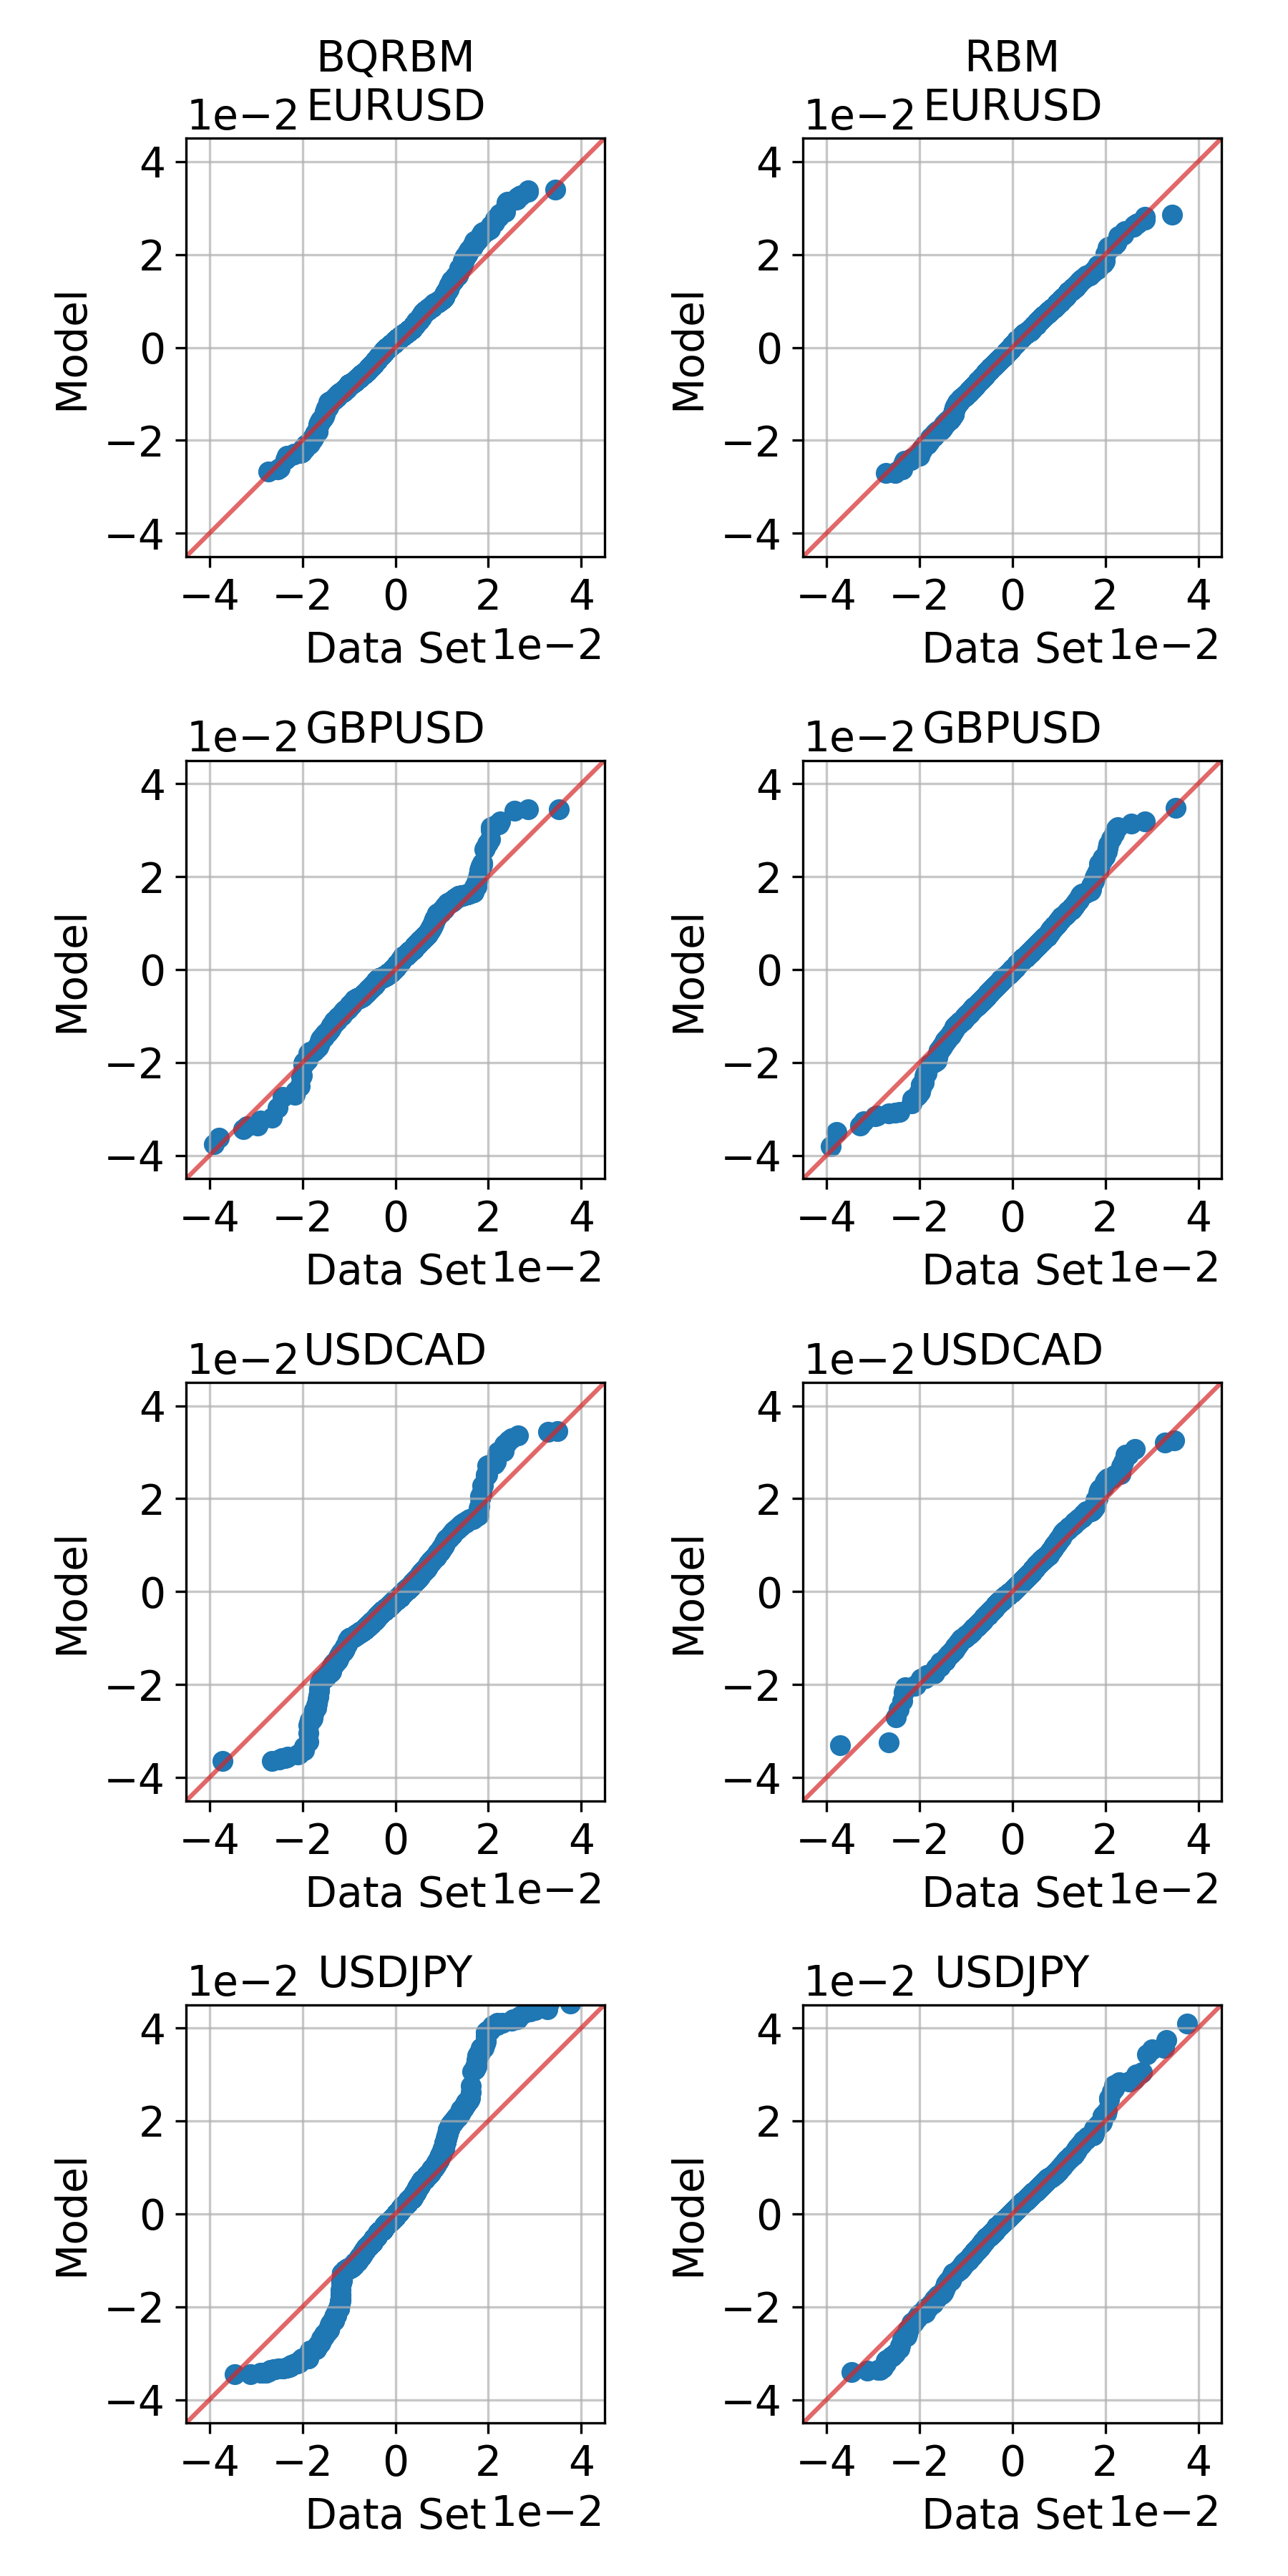
\includegraphics[width=1\linewidth]{rbm/qq.png}
    \end{center}
    \caption{Log return Q-Q plots of the RBM models for each currency pair. Note that these plots only use the same number of samples as the size of the training data set (5165), and thus are not entirely representative of the models' performances.}
    \label{fig:rbm_qq_plots}
\end{figure}

\subsubsection{Correlations}
The distribution is in a sense more than just the sum of its parts.
Beyond learning the marginal distributions, the models should also capture the correlations between the currency pairs.
To verify this, we turn to the correlation coefficients in~\cref{tbl:rbm_correlation_coefficients} to see how well the models capture the correlations.
We find that the models reproduce the structure of the correlation coefficients reasonably well, with the models trained on the transformed data sets encoding more of the behavior.
\begin{table}[!htb]
    \centering
    \begin{adjustbox}{max width=\textwidth}
        \input{../tables/rbm/correlation_coefficients.tbl}
    \end{adjustbox}
    \caption{Correlation coefficients of the data set vs.~samples generated by the RBM models. The RBM values are shown in the format mean \(\pm\) one standard deviation from an ensemble of 100 sample sets consisting of \( 10^4 \) samples each.}
    \label{tbl:rbm_correlation_coefficients}
\end{table}

\subsubsection{Volatilities}
Examining the historical volatilities in~\cref{tbl:rbm_volatilities} confirms the models can produce synthetic data with similar volatilities to the training data set, albeit marginally higher in all cases.
\begin{table}[!htb]
    \centering
    \begin{adjustbox}{max width=\textwidth}
        \input{../tables/rbm/volatilities.tbl}
    \end{adjustbox}
    \caption{Historical volatilities of the data set vs.~samples generated by the RBM models. The RBM values are shown in the format mean \(\pm\) one standard deviation from an ensemble of 100 sample sets consisting of \( 10^4 \) samples each.}
    \label{tbl:rbm_volatilities}
\end{table}

\subsubsection{Tails}
It is extremely important for the models to learn the tail events because these play a crucial role in financial risk management.
The models trained on the transformed data sets reproduce the lower tails a little better for most currency pairs, but overestimate some of the upper tails.
It is difficult to say overall if one model performs better than another here, as it really depends on what one wants to do with the generated data.
\begin{table}[!htb]
    \centering
    \begin{adjustbox}{max width=\textwidth}
        \input{../tables/rbm/tails.tbl}
    \end{adjustbox}
    \caption{Lower and upper tails, i.e., 1st and 99th percentiles, of the data set vs.~samples generated by the RBM models. The RBM values are shown in the format mean \(\pm\) one standard deviation from an ensemble of 100 sample sets consisting of \( 10^4 \) samples each.}
    \label{tbl:rbm_tails}
\end{table}

We also study the tail concentration functions (see~\cref{app:tail_concentration_functions} for definitions and interpretations) between currency pairs in~\cref{fig:rbm_tail_concentrations}.
Here we see that all models perform quite well for the most part except for a few of the extreme regions in the EURUSD/GBPUSD, EURUSD/USDJPY, and GBPUSD/USDJPY plots.
\begin{figure}[!htb]
    \begin{center}
        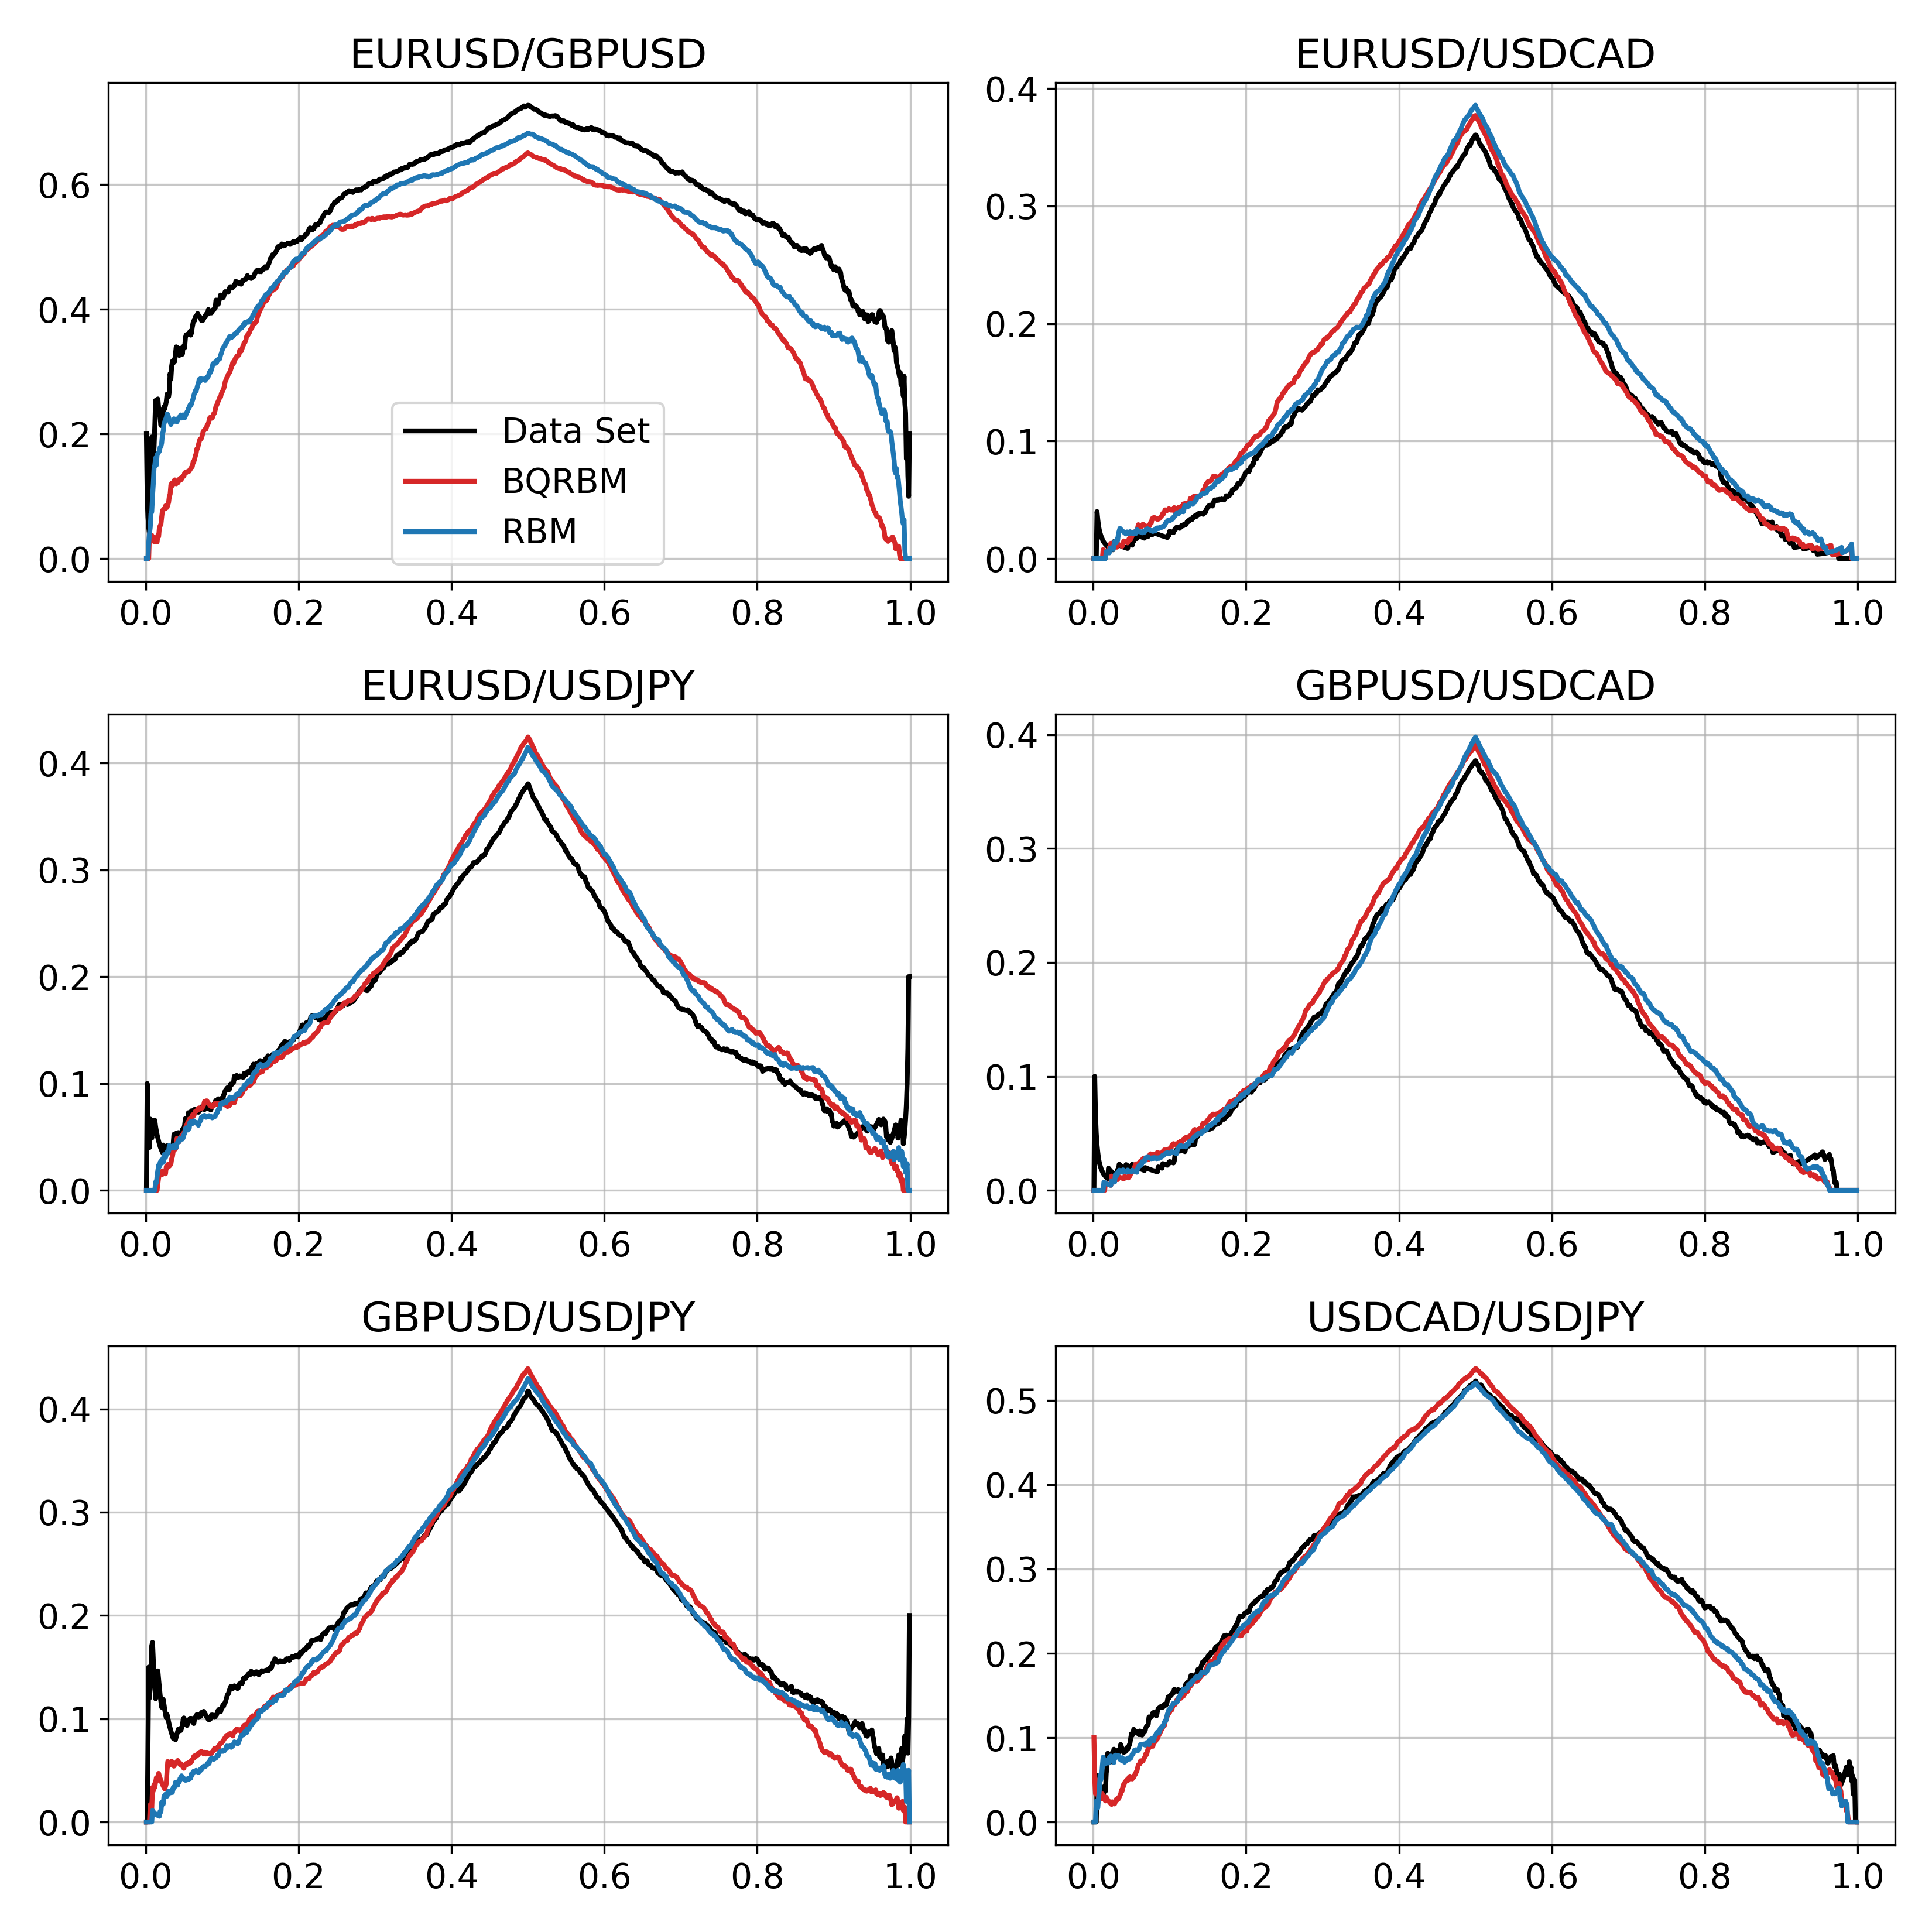
\includegraphics[width=1\linewidth]{rbm/tail_concentrations.png}
    \end{center}
    \caption{Tail concentration functions of the data set vs.~samples generated by the RBM models.}
    \label{fig:rbm_tail_concentrations}
\end{figure}

\subsubsection{Conditional Sampling}
One of the advantages of the RBM is its ability to perform conditional sampling.
For the data sets with additional volatility indicators, we have the ability to condition on these indicators to sample from a specific volatility regime.
This is useful, for example, if we are trying to generate real-world data that fits the current volatility landscape.

This leads us to look at the conditional volatilities, i.e., seeing how well the models reproduce the volatilities from the two volatility regimes.
Laid out in~\cref{tbl:rbm_conditional_volatilities}, we observe that the samples produced by the RBMs have slightly lower (higher) volatilities in the high (low) regime, but are overall in good agreement with the data set.
\begin{table}[!htb]
    \centering
    \begin{adjustbox}{max width=\textwidth}
        \input{../tables/rbm/conditional_volatilities.tbl}
    \end{adjustbox}
    \caption{Conditional historical volatilities of the data set vs.~samples generated by the RBM models. The RBM values are shown in the format mean \(\pm\) one standard deviation from an ensemble of 100 sample sets consisting of \( 10^4 \) samples each.}
    \label{tbl:rbm_conditional_volatilities}
\end{table}

\subsection{Summary}
The classical RBM results presented in this section are in line with those obtained by Kondratyev and Schwarz in~\cite{kondratyev_2019}, and the differences can likely be accounted for by the different data sets used in training (e.g., different sources, different filtering, etc.), model hyperparameters, and the stochastic nature of the models.
This further confirms that the RBM is performant and can be used to generate synthetic data from distributions with intricate structures, such as the correlations and volatilities seen here.

Overall it is difficult to say if one of the models performs better than the others, as it depends on the desired use case, but the models trained on the transformed data sets do yield lower KL divergence values and capture more of the correlations between currency pairs.
This offers evidence that the results might be able to be further improved through the use of more advanced data preprocessing methods.
We do not investigate these possibilities any further though, given that this is not the main scope of this thesis.
The results in this section act mainly as a point of reference to compare the quantum models within the next chapter.
